\documentclass{tufte-handout}

\title{Propositional Probability II: Reasoning\thanks{CS7470 Fall 2023: Foundations of Probabilistic Programming.}}



\author[]{Steven Holtzen\\s.holtzen@northeastern.edu}

%\date{28 March 2010} % without \date command, current date is supplied

%\geometry{showframe} % display margins for debugging page layout
\setcounter{secnumdepth}{1}

\usepackage{graphicx} % allow embedded images
  \setkeys{Gin}{width=\linewidth,totalheight=\textheight,keepaspectratio}
  \graphicspath{{graphics/}} % set of paths to search for images
\usepackage{amsmath,amssymb,amsthm}  % extended mathematics
\usepackage{booktabs} % book-quality tables
\usepackage{units}    % non-stacked fractions and better unit spacing
\usepackage{multicol} % multiple column layout facilities
\usepackage{lipsum}   % filler text
\usepackage{fancyvrb} % extended verbatim environments
  \fvset{fontsize=\normalsize}% default font size for fancy-verbatim environments
\usepackage{listings}
\usepackage{tikz}
\usepackage{mathpartir}
\usepackage{subcaption}
\usepackage{mdframed}
\usepackage{epigraph}
\usepackage{enumitem}
\usepackage{stmaryrd}

\usetikzlibrary{shapes.geometric}


\usepackage[ruled,linesnumbered]{algorithm2e}
\SetKwComment{Comment}{/* }{ */}
\newcommand{\indep}{\perp \!\!\! \perp}

\tikzset{
  treenode/.style = {shape=rectangle, rounded corners,
                     draw, align=center,
                     },
  root/.style     = {treenode, font=\Large, bottom color=red!30},
  env/.style      = {treenode, font=\ttfamily\normalsize},
  dummy/.style    = {circle,draw}
}

% tikz
\usetikzlibrary{patterns,calc,backgrounds}


% TIKZ
\tikzstyle{nnf}=[
  >=stealth,font=\small,auto,scale=0.7,every node/.style={scale=0.7}
]
\tikzstyle{extnode}=[
  draw,circle,inner sep=2pt,fill=white
]

\tikzstyle{leafnode}=[
  draw,fill=gray!20,inner sep=3.5pt
]
\tikzstyle{constnode}=[
  draw,fill=white,inner sep=3.5pt
]
\tikzstyle{label}=[
  fill=white,inner sep=2.5pt
]

\tikzstyle{acarrow}=[
    decoration={markings,mark=at position 1 with {\arrow[scale=0.6]{>}}},
    postaction={decorate},
    shorten >=0.4pt,
    >=latex,
    line width=0.1
]

\tikzstyle{bnarrow}=[
    decoration={markings,mark=at position 1 with {\arrow[scale=1.5]{>}}},
    postaction={decorate},
    shorten >=0.7pt,
    >=latex,
    line width=0.3
]
\tikzstyle{bayesnet}=[
  >=latex, thick, auto
]
\tikzstyle{bnnode}=[
  draw,ellipse,minimum size=7mm,inner sep=1pt,font=\small
]
\tikzstyle{cpt}=[
  font=\footnotesize
]

\tikzstyle{graph}=[
  >=stealth,font=\small,auto,scale=1,every node/.style={scale=1}
]
\tikzstyle{node}=[
  draw,circle,inner sep=3pt,fill=white
]

% BDDs

\tikzstyle{bdd}=[
  >=latex, thick, >=stealth, font=\small,auto,scale=0.9,every node/.style={scale=0.9}
]
\tikzstyle{bddnode}=[
  draw,circle,inner sep=0pt,fill=white,minimum size=5.5mm
]

\tikzstyle{bddtriangle}=[
  draw, regular polygon, regular polygon sides = 3,inner sep=1pt,fill=white,minimum size=5.5mm
]

\tikzstyle{highedge}=[
    line width=0.9
]
\tikzstyle{lowedge}=[
    line width=0.9,dotted
]
\tikzstyle{bddterminal}=[
  draw,fill=gray!20,inner sep=2.5pt, font=\small
]

\lstdefinestyle{compact}{
  \ttfamily\tiny
}


\usetikzlibrary{positioning}

\newtheorem{theorem}{Theorem}
\newtheorem{definition}{Definition}
\newtheorem{conjecture}{Conjecture}
\newtheorem{lemma}{Lemma}
\newtheorem{exercise}{Exercise}
\newtheorem{remark}{Remark}


\usepackage{xcolor}

\definecolor{codegreen}{rgb}{0,0.6,0}
\definecolor{codegray}{rgb}{0.5,0.5,0.5}
\definecolor{codepurple}{rgb}{0.58,0,0.82}
\definecolor{backcolour}{rgb}{0.95,0.95,0.92}

\lstdefinestyle{mystyle}{
    backgroundcolor=\color{backcolour},   
    commentstyle=\color{codegreen},
    keywordstyle=\color{magenta},
    numberstyle=\tiny\color{codegray},
    stringstyle=\color{codepurple},
    basicstyle=\ttfamily\footnotesize,
    breakatwhitespace=false,         
    breaklines=true,                 
    captionpos=b,                    
    keepspaces=true,                 
    numbers=left,                    
    numbersep=5pt,                  
    showspaces=false,                
    showstringspaces=false,
    showtabs=false,                  
    tabsize=2
}

\lstset{style=mystyle}

\newcommand{\defn}[1]{\textbf{#1}}
\newcommand{\dbracket}[1]{\left \llbracket {#1} \right \rrbracket}
\newcommand{\dist}[1]{\mathtt{Dist}(#1)}
\newcommand{\true}[0]{\texttt{true}}
\newcommand{\te}[0]{\texttt{e}}
\newcommand{\false}[0]{\texttt{false}}
\newcommand{\real}[0]{\mathbb{R}}
\newcommand{\rational}[0]{\mathbb{Q}}
\newcommand{\lebesgue}[0]{\mathbb{L}}
\newcommand{\eval}[0]{\mathrm{ev}}
\newcommand{\disc}[0]{\textsc{Disc}}
\newcommand{\borel}[0]{\mathcal{B}}
\newcommand{\ent}[0]{\mathbb{S}}
\newcommand{\prog}[0]{\texttt{p}}
\newcommand{\bool}[0]{\mathbb{B}}
\newcommand{\cont}[0]{\textsc{Cont}}
\newcommand{\prop}[0]{\textsc{Prop}}
\newcommand{\bdd}[0]{\textsc{Bdd}}
\newcommand{\robdd}[0]{\textsc{Robdd}}
\newcommand{\compiles}[0]{\rightsquigarrow}

\newcommand{\bddtriangle}[1]{
    \begin{tikzpicture}
    \node [bddtriangle] {#1};
    \end{tikzpicture}}
\newcommand{\bddtrue}[0]{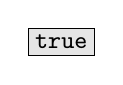
\begin{tikzpicture}
      \node [bddterminal] {$\true$};
    \end{tikzpicture}}
\newcommand{\bddfalse}[0]{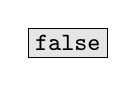
\begin{tikzpicture}
      \node [bddterminal] {$\false$};
    \end{tikzpicture}}


% Standardize command font styles and environments
\newcommand{\doccmd}[1]{\texttt{\textbackslash#1}}% command name -- adds backslash automatically
\newcommand{\docopt}[1]{\ensuremath{\langle}\textrm{\textit{#1}}\ensuremath{\rangle}}% optional command argument
\newcommand{\docarg}[1]{\textrm{\textit{#1}}}% (required) command argument
\newcommand{\docenv}[1]{\textsf{#1}}% environment name
\newcommand{\docpkg}[1]{\texttt{#1}}% package name
\newcommand{\doccls}[1]{\texttt{#1}}% document class name
\newcommand{\docclsopt}[1]{\texttt{#1}}% document class option name
\newenvironment{docspec}{\begin{quote}\noindent}{\end{quote}}% command specification environment



\begin{document}
\maketitle% this prints the handout title, author, and date


Now we are ready to return to our earlier discussion and ask: \emph{can we use
propositional logic as the basis for an effective probabilistic model}?
The first question is: what is our sample space? It's clear so far that a logical 
choice of sample space is the set of all possibly instances for a fixed set 
of Boolean formulae; this sample space will have size $2^n$, where $n$ is the number 
of propositional variables.
Now, if we want to efficiently evaluate queries over this sample space, we need
need two more components:
\begin{enumerate}
    \item A way to efficiently represent a probability distribution on the sample space;
    \item A way to efficiently represent queries over that sample space.
\end{enumerate}

Let's tackle (1) first. What is an alternative representation of a distribution 
that avoids the space-explosion we saw in the lookup-table representation? We 
will need to be more clever about how we represent probabilities. One useful
choice is to assume that all random variables are \emph{independent from each other}, 
and therefore we can concisely describe a joint distribution over all of them:

\begin{definition}[Fully factorized probabilistic model]
    Let $X_1, X_2, \cdots, X_n$ be jointly independent random variables (i.e.,
    for any pair $X_i, X_j$, it is the case that $X_i \indep X_j$). Then, a
    fully-factorized probabilistic model is a collection of $n$ probability
    lookup tables $\Pr(X_i)$, one for each $i$. The joint probability is computed 
    as $\Pr(X_1, X_2, \cdots, X_n) \triangleq \prod_i^n \Pr(X_i)$.
\end{definition}

Observe that a fully-factorized model only requires $O(\sum_i |X_i|)$ space,
which is significantly smaller than $|\Omega|$.\sidenote{The notation $|X|$
refers to the size of a random variable's co-domain.} This is a big improvement
over plain lookup tables, but it comes at a cost of expressivity: there are some
distributions that cannot be represented in a fully-factorized way.

In the context of propositional logic, there is a natural notion of a
fully-factorized model. Let $\Omega$ be the collection of $n$-element instances.
Then, each propositional variable corresponds to a projection out of that sample
space. Let's call this the \defn{fully factorized propositional distribution}: each 
variable in the theory will be associated with an independent probability of 
being $\true$ or $\false$. For example, we may have to propositional variables $x$ and 
$y$; the fully factorized distribution could be given by two independent lookup tables:
\begin{align}
    [x \mapsto 0.1, \overline{x} \mapsto 0.9], \quad [y \mapsto 0.2, \overline{y} \mapsto 0.8].
    \label{eq:indepdist}
\end{align}
Then, the joint probability $\Pr(x, \overline{y})$ is $0.1 \times 0.8$.

\newthought{Now we return to an earlier question}: how do we efficiently represent 
events in the propositional setting? Events are a subset of the sample space. 
The sample space in propositional probability is the set of all instances. Then, 
we can represent events by \emph{propositional formulae}:
\begin{align}
    \Pr(\varphi) \triangleq \sum_{I \models \varphi} \Pr(\varphi).
\end{align}
For instance, for the fully-factorized 
distribution in Eq.~\ref{eq:indepdist}, we can compute the probability of a 
propositional sentence $x \lor y$ by summing the probability mass over each 
instance that models this formula:
\begin{align}
    \Pr(x \lor y) = \Pr([x, y]) + \Pr([x, \overline{y}]) + \Pr(\overline{x}, y).
\end{align}

This is implemented by the following algorithm:

\begin{algorithm}
    \caption{QueryPropositionalEvent$_1$($\Pr, \varphi)$}
    \KwData{A fully-factorized distribution $\Pr$; a propositional formula $\varphi$}
    \KwResult{The probability of the event $\Pr(\varphi)$}
    $a \leftarrow 0$\;
    \For{each $I \in \Omega$}{
        \lIf{$I \models \varphi$}{$a \leftarrow a + \Pr(\omega)$}
    }
    \Return{a}
    \label{alg:enum}
\end{algorithm}


Unfortunately, QueryPropositionalEvent is \emph{still linear} in the size of
$|\Omega|$ due to the outer loop on Lines 2--4.  In all cases, regardless of the
structure of $\varphi$, we have to consider all all the instances, which will
not scale. 

\subsection{Efficiently evaluating queries via search}
How do we avoid scaling in $|\Omega|$ during querying? 
In other words: is it possible to design a scalable automated reasoning strategy 
for our tiny probabilistic programming language that we've made so far, with fully-factorized 
propositional distributions and queries given as propositional formulae?
In the worst case, it
may not be possible to avoid considering all possible instances, but we can 
try to avoid this worst-case explosion by delicately \emph{exploiting the problem 
structure}: in particular, we want to simultaneously exploit the fully-factorized 
structure of the distribution along with the fact that all events are written 
as propositional formulae.

One approach is to \emph{exploit the structure of models of the query
$\varphi$}: sometimes, a query may only have a single model, or perhaps most
instances are models. In these cases, we waste a lot of effort enumerating all
models; it is much more efficient to \emph{search} for the few satisfying instances.

For example, consider the formula $x \lor y$. We can recursively decompose this
formula by branching on assignments to propositional variables:

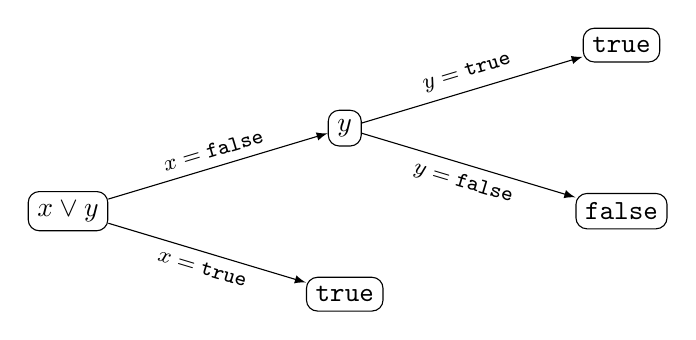
\begin{tikzpicture}
    [
      grow                    = right,
      sibling distance        = 6em,
      level distance          = 10em,
      edge from parent/.style = {draw, -latex},
      every node/.style       = {font=\footnotesize},
      sloped
    ]
    \node [env] {$x \lor y$}
      child { node [env] {$\true$}
        edge from parent node [below] {$x = \true$} }
      child { node [env] {$y$}
        child { node [env] {$\false$}
          edge from parent node [below] {$y = \false$} }
        child { node [env] {$\true$}
                edge from parent node [above, align=center]
                  {$y = \true$}}
                edge from parent node [above] {$x = \false$} };
  \end{tikzpicture}

The root of this binary tree is the original formula $x \lor y$. Each branch 
assigns a propositional variable to a Boolean value. The children are 
the resulting formula evaluated on the \emph{partial instance} given by the 
path up until that point: for instance, if we assign $x = \false$, we are left 
with the formula $\false \lor y = y$. Leaves of the tree denote whether or not a 
particular assignment is a model.\sidenote{% source: https://tex.stackexchange.com/questions/188183/latex-under-construction-in-work-or-work-in-progress-symbols
\scalebox{0.5}[0.5]{
    (under construction)

\begin{tikzpicture}[limb/.style={line cap=round,line width=1.5mm,line join=bevel}]
\draw[line width=2mm,rounded corners,fill=yellow] (-2,0) -- (0,-2) -- (2,0) -- (0,2) -- cycle;
\fill (1.5mm,7mm) circle (1.5mm);
\fill(0,-7.5mm) -- ++(10mm,0mm) -- ++(120:2mm)--++(100:1mm)--++(150:2mm) arc (70:170:2.5mm and 1mm);
\draw[limb] (-7.5mm,-6.5mm)--++(70:4mm)--++(85:4mm) coordinate(a)--++(-45:5mm)--(-2.5mm,-6.5mm);
\fill[rotate around={45:(a)}] ([shift={(-0.5mm,0.55mm)}]a) --++(0mm,-3mm)--++
        (7mm,-0.5mm)coordinate(b)--++(0mm,4mm)coordinate(c)--cycle;
\draw[limb] ([shift={(-0.6mm,-0.4mm)}]b) --++(-120:5mm) ([shift={(-0.5mm,-0.5mm)}]c) --++
        (-3mm,0mm)--++(-100:3mm)coordinate (d);
\draw[ultra thick] (d) -- ++(-45:1.25cm);
\end{tikzpicture}
}}

% this can be described using big-step!
\begin{algorithm}
    \caption{PrEvent($\Pr, \varphi$)}
    \KwData{A fully-factorized distribution $\Pr$; a propositional formula $\varphi$; a decision order $\sigma$.}
    \KwResult{The probability $\Pr(\varphi)$.}
    \lIf{$\varphi = \true$}{\Return 1}
    \lIf{$\varphi = \false$}{\Return 0}
    $v \leftarrow head(\sigma)$\;
    $\sigma' \leftarrow tail(\sigma)$\;
    $ \varphi_v \leftarrow $ fix $v = \true$ in $\varphi$\;
    $ \varphi_{\overline{v}} \leftarrow $ fix $v = \false$ in $\varphi$\;
    \Return{$\Pr(v) \times $PrEvent$(\Pr, \varphi_v) + \Pr(\overline{v}) \times $PrEvent$(\Pr, \varphi_{\overline{v}})$}
    \label{alg:rec}
\end{algorithm}

You should convince yourself that the above algorithm is correct by trying it on a few examples. 
It is a good exercise to prove it correct inductively.
What is the runtime of Algorithm~\ref{alg:rec}? In the worst-case, it is still $|\Omega|$. But, 
sometimes -- depending on the structure of $\varphi$ -- it can do better by terminating the 
recursion earlier in a base-case on Lines 1 and 2, rather than exhaustively exploring all 
instances like Algorithm~\ref{alg:enum}.



% Now, suppose we are given a probability measure $\Pr$ on instances. Now we want
% to ask: \emph{what is the probability that a particular sentence $\varphi$ is
% true for this world?} A subset of $\Omega$ is called an \defn{event}, and the 
% probability of this particular event can be computed as the total probability of
% all models of $\varphi$:
% \begin{align}
%     \Pr(\varphi) \triangleq \sum_{I \models \varphi} \Pr(I).
%     \label{eq:pr2}
% \end{align}
% Note that above we overloaded the notation used for $\Pr$ to now act 
% on events; this is common practice.
% As an example, using the probability measure given in Table~\ref{tbl:simple}, we
% can compute:
% \begin{align}
% \Pr(x \lor y) = \Pr([x, y]) + \Pr([x, \overline{y}]) + \Pr(\overline{x}, y) = 0.6.
% \end{align}

% \subsection{A propositional probabilistic programming language}
% Tables like Table~\ref{tbl:simple} are a very inconvenient way to describe a
% probability distribution. They are exponential in size, making them infeasible 
% to write down for a large set of propositional variables, and they convey no useful 
% structure to the user. In short, tables aren't a very useful probabilistic 
% programming language.

% It is much more convenient and usable 

\begin{exercise}[$\star$]
    Assume the following fully-factorized distribution on propositional variables:
    \begin{align*}
        [x \mapsto 0.1, \overline{x} \mapsto 0.9],\quad [y \mapsto 0.3, \overline{y} \mapsto 0.7].
    \end{align*}
    Use an exhaustive search tree to compute $\Pr(x \Leftrightarrow y)$.
\end{exercise}
\begin{exercise}[$\star\star$]
    Prove Algorithm~\ref{alg:rec} correct.
\end{exercise}


\bibliographystyle{plainnat}
\bibliography{../bib}

\end{document}